\documentclass[10pt,a4paper,fleqn]{article}
\setlength{\oddsidemargin}{-1.4mm}
\setlength{\evensidemargin}{-1.4mm}
\setlength{\textwidth}{162mm}
\setlength{\topmargin}{-12mm}
\setlength{\textheight}{249mm}
\usepackage{amsmath,amssymb,bm,booktabs,array}
\usepackage{xcolor,graphicx,tikz,pgfplots}
\usepackage{url}
% Clickable, breakable URLs using pdfTeX primitives; no hyperref dependency.
\let\plainurl\url
\renewcommand{\url}[1]{\ifdefined\pdfstartlink\leavevmode\pdfstartlink attr{/Border [0 0 0]} user{/Subtype /Link /A << /S /URI /URI (\pdfescapestring{#1}) >>}\plainurl{#1}\pdfendlink\else\plainurl{#1}\fi}
\pgfplotsset{compat=1.18}
\newif\ifmarked
\markedfalse
\definecolor{revisionblue}{RGB}{18,61,130}
\newcommand{\rev}[1]{{\ifmarked\color{revisionblue}\else\color{black}\fi #1}}
\newenvironment{revision}{\begingroup\ifmarked\color{revisionblue}\else\color{black}\fi\nobreak\ignorespaces}{\par\endgroup}
\newcommand{\Eavg}{\overline{\mathcal E}_h}
\newcommand{\Cstep}{\mathcal C}
\newcommand{\Rstep}{\mathcal R}
\newcommand{\mean}[1]{\overline{#1}}
\setlength{\textfloatsep}{14pt plus 3pt minus 2pt}
\setlength{\intextsep}{14pt plus 3pt minus 2pt}
\renewcommand{\topfraction}{0.9}
\renewcommand{\textfraction}{0.08}
\renewcommand{\floatpagefraction}{0.75}
\raggedbottom
\setlength{\emergencystretch}{1em}
\pagestyle{empty}
\makeatletter
\newlabel{eq:ch}{{1}{2}{}{equation.1}{}}
\newlabel{eq:energy}{{2}{2}{}{equation.2}{}}
\newlabel{eq:structure}{{3}{2}{}{equation.3}{}}
\newlabel{eq:step}{{4}{3}{}{equation.4}{}}
\newlabel{eq:fit}{{5}{3}{}{equation.5}{}}
\newlabel{eq:ridge}{{6}{3}{}{equation.6}{}}
\newlabel{eq:candidate}{{7}{3}{}{equation.7}{}}
\newlabel{eq:discreteenergy}{{8}{3}{}{equation.8}{}}
\newlabel{eq:derivatives}{{9}{3}{}{equation.9}{}}
\newlabel{eq:massproj}{{10}{4}{}{equation.10}{}}
\newlabel{eq:accept}{{11}{4}{}{equation.11}{}}
\newlabel{eq:backtrack}{{12}{4}{}{equation.12}{}}
\newlabel{eq:descent}{{13}{4}{}{equation.13}{}}
\newlabel{eq:galerkinenergy}{{14}{5}{}{equation.14}{}}
\newlabel{eq:galerkinlaw}{{15}{5}{}{equation.15}{}}
\newlabel{eq:pidmd}{{16}{5}{}{equation.16}{}}
\newlabel{eq:adaptive}{{17}{5}{}{equation.17}{}}
\newlabel{eq:initial}{{18}{6}{}{equation.18}{}}
\newlabel{eq:errors}{{19}{7}{}{equation.19}{}}
\newlabel{eq:structureerror}{{20}{7}{}{equation.20}{}}
\newlabel{eq:violation}{{21}{7}{}{equation.21}{}}
\newlabel{eq:rectangles}{{22}{7}{}{equation.22}{}}
\newlabel{tab:accuracy}{{1}{8}{}{table.1}{}}
\newlabel{tab:epsilon}{{2}{10}{}{table.2}{}}
\newlabel{tab:mobility}{{3}{10}{}{table.3}{}}
\newlabel{tab:long}{{4}{11}{}{table.4}{}}
\newlabel{tab:timing}{{5}{12}{}{table.5}{}}
\newlabel{eq:cost}{{23}{13}{}{equation.23}{}}
\newlabel{tab:convergence}{{6}{13}{}{table.6}{}}
\newlabel{tab:teacher}{{7}{14}{}{table.7}{}}
\newlabel{tab:finer}{{8}{15}{}{table.8}{}}
\newlabel{tab:crossgrid}{{9}{15}{}{table.9}{}}
\newlabel{tab:deterministic}{{10}{15}{}{table.10}{}}
\newlabel{tab:hyper}{{11}{17}{}{table.11}{}}
\newlabel{tab:shifts}{{12}{17}{}{table.12}{}}
\newlabel{eq:fixedfilterlimit}{{24}{18}{}{equation.24}{}}
\makeatother
\begin{document}
\setcounter{figure}{5}
\begin{figure}[htbp]\centering
\begin{tikzpicture}
\begin{axis}[width=.78\textwidth,height=5.4cm,grid=major,grid style={gray!15},tick label style={font=\footnotesize},label style={font=\small},xlabel={$N$},ylabel={Relative field difference},title style={font=\small},legend style={font=\scriptsize,draw=none},legend pos=south west,xtick={64,128,256},xticklabels={64,128,256},xmode=log,ymode=log]
\addplot[thick,solid,mark=*,mark size=2pt,mark options={solid},blue!65!black] coordinates {(64,0.0424066554) (128,0.000789687958) (256,5.72430803e-07)};
\addlegendentry{Random, $t=0.0035$}
\addplot[thick,dashed,mark=square*,mark size=2pt,mark options={solid},orange!85!black] coordinates {(64,0.451661725) (128,0.132022387) (256,0.00241654403)};
\addlegendentry{Random, $t=0.07$}
\addplot[thick,dashdotted,mark=triangle*,mark size=2pt,mark options={solid},teal!80!black] coordinates {(64,0.0346830218) (128,0.00476309301) (256,0.000118902369)};
\addlegendentry{Rectangles, $t=0.0035$}
\addplot[thick,densely dotted,mark=diamond*,mark size=2pt,mark options={solid},purple] coordinates {(64,0.0625388958) (128,0.0138930523) (256,0.000652334913)};
\addlegendentry{Rectangles, $t=0.07$}
\end{axis}
\end{tikzpicture}
\rev{\caption{\rev{Spatial relative field differences against the $512^2$ dealiased ETDRK4 solution after Fourier interpolation of each coarser field, at $\epsilon=0.020$ and $M=1$. Random polynomial case zero uses blue solid circles at $t=0.0035$ and orange dashed squares at $t=0.070$; the deterministic rectangles use teal dash-dot triangles and purple dotted diamonds at the corresponding times. Each point represents one initial field, with no ensemble uncertainty implied. The temporal step is at most $5\times10^{-5}$; time refinement is assessed separately. Table~\ref{tab:convergence} reports adjacent-grid differences, whereas this plot uses $512^2$ as the common comparison grid. Intermediate times and additional random fields are retained in the supplementary data.}}\label{fig:convergence}}
\end{figure}
\clearpage
\end{document}
